\clearpage

\lehead[]{\sf\hspace*{-2.00cm}\textcolor{white}{\colorbox{lightblue}{\parbox[c][0.70cm][b]{1.60cm}{
\makebox[1.60cm][r]{\thechapter}\\ \makebox[1.60cm][r]{ÜBUNG}}}}\hspace{0.17cm}\textcolor{lightblue}{\chaptertitle}}
\rohead[]{\textcolor{lightblue}{\chaptertitle}\sf\hspace*{0.17cm}\textcolor{white}{\colorbox{lightblue}{\parbox[c][0.70cm][b]{1.60cm}{\thechapter\\
ÜBUNG}}}\hspace{-2.00cm}}
%\chead[]{}
\rehead[]{\textcolor{lightblue}{AvHG, Inf, My}}
\lohead[]{\textcolor{lightblue}{AvHG, Inf, My}}

\section{Typkonvertierungen -- Übungen}

\subsection{Aufgabe 1: Typkonvertierungen}

Kopiere in den nachfolgenden Teilaufgaben jeweils die obere Variable in die
untere Variable, in dem du den Typ der Variablen geeignet konvertierst. Welcher
Wert wird nach der Konvertierung in der zweiten Variablen stehen? Welche
Konvertierungen sind erlaubt, welche führen zu einem Systemfehler? Teste deine
Lösung in Eclipse aus.

\begin{compactenum}[a)]
\item 
\begin{lstlisting}
char c = 'A';
int zahl = 
\end{lstlisting}

\item 
\begin{lstlisting}
int zahl = 65;
char c =
\end{lstlisting}

\item 
\begin{lstlisting}
boolean b = true;
int zahl =
\end{lstlisting}

\item 
\begin{lstlisting}
String text = "Hallo";
int zahl =
\end{lstlisting}

\item 
\begin{lstlisting}
int zahl = 65;
String text =
\end{lstlisting}

\item 
\begin{lstlisting}
char c = 'A';
String text =
\end{lstlisting}

\item 
\begin{lstlisting}
JButton btn = new JButton("Drück mich");
JLabel lbl =
\end{lstlisting}

\item 
\begin{lstlisting}
J(h) JButton btn = new JButton("Drück mich");
Object obj = (Object) b;
JTextField tf =
\end{lstlisting}
\end{compactenum}


\subsection{Aufgabe 2: Tic Tac Toe}

Programmiere eine einfache Version des Spiels Tic Tac Toe.

\begin{minipage}{0.5\textwidth}
Oberfläche zu Beginn des Spiels:

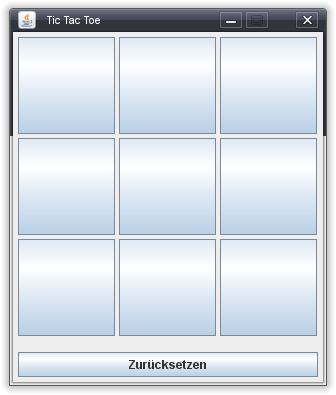
\includegraphics[width=0.8\textwidth]{./inf/SEKII/24_Java_GUI-Komponenten/TicTacToe_1.png}
\end{minipage}
\begin{minipage}{0.5\textwidth}
Oberfläche während des Spiels:

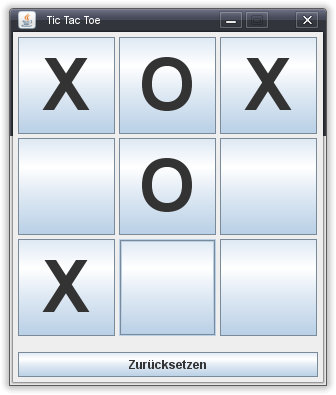
\includegraphics[width=0.8\textwidth]{./inf/SEKII/24_Java_GUI-Komponenten/TicTacToe_2.png}       
\end{minipage}

Das Spielfeld wird als ein Array von neun Buttons dargestellt, die zu Beginn
keinen Text enthalten. Wenn man auf einen Button drückt, erhalten die Buttons
immer abwechselnd den String \glqq X\grqq\ oder \glqq O\grqq\ als Aufschrift.

Wenn der Zurücksetzen-Button gedrückt wird, erhalten alle Buttons einen leeren
String als Aufschrift, damit das Spiel von vorne beginnen kann. Mehr braucht
die einfache Spiel-Version nicht zu können.

Zusatzaufgabe:

\begin{compactenum}[a)]
\item Überprüfe zusätzlich die Korrektheit der Eingabe und gib eine
Fehlermeldung aus, wenn ein Button gedrückt wird, der schon einen Text enthält.

\item Überprüfe, ob einer der Spieler gewonnen hat und gib gegebenenfalls eine
entsprechende Meldung aus.
\end{compactenum}


\subsection{Aufgabe 3: Taschenrechner}

Programmiere einen sehr vereinfachten Taschenrechner.

\begin{center}
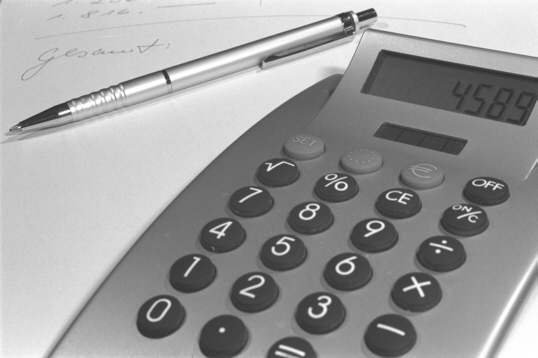
\includegraphics[width=0.6\textwidth]{./inf/SEKII/24_Java_GUI-Komponenten/Taschenrechner.png}
% Copyright??
\end{center}

\begin{compactenum}[a)]
\item Im ersten Schritt sollen nur Zahlen zwischen 1 und 9 addiert werden
können. Der Taschenrechner besteht aus folgenden Komponenten:

\begin{compactitem}
\item Ein JTextField zur Ausgabe der aktuellen Summe. Es soll dem Benutzer
unmöglich sein, in dem Textfeld Eingaben vorzunehmen.
\item Ein Array von zehn Buttons zur Eingabe der Zahlen von 0 bis 9 (Es ist
einfacher die Null mit einzubeziehen, auch wenn sie in Teilaufgabe a) noch
nicht benötigt wird).
\item Einen Reset-Button, mit dem die Summe auf 0 zurück gesetzt werden kann. 
\end{compactitem}

Wenn der Benutzer einen der Zahlen-Button drückt, wird die Summe im Textfeld um
den Wert der entsprechenden Zahl erhöht.

\item Erweitere den Taschenrechner so, dass auch zusammengesetzte Zahlen
addiert werden können (z.B. 46 + 333). Füge Buttons für eine Plus-Taste (+) und
eine Gleich-Taste (=) hinzu.

Wenn Zahlen-Tasten gedrückt werden, sollen die Ziffern (wie bei einem normalen
Taschenrechner) an die aktuell angezeigte Zahl angehängt werden. Beim Drücken
der Plus-Taste wird die angezeigte Zahl zu der intern abgespeicherten Summe
dazu addiert und das Textfeld wird für die nächste Zahl gelöscht. Wenn der
Benutzer die Gleich-Taste drückt, wird die aktuelle Zahl zu der internen Summe
dazu addiert und die Summe ausgegeben.

Das nachfolgende Zustandsdiagramm veranschaulicht die Funktionsweise des
Taschenrechners:

\begin{center}
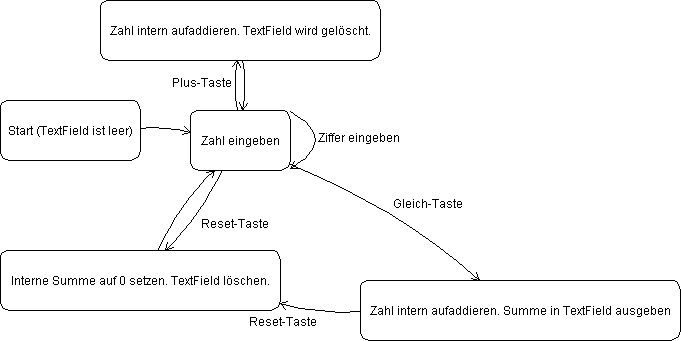
\includegraphics[width=0.9\textwidth]{./inf/SEKII/24_Java_GUI-Komponenten/Taschenrechner-Zustandsdiagramm.png}
\end{center}

\item Erweitere den Taschenrechner um eine Minus-Taste (-), eine
Multiplikations-Taste (x) und eine Divisions-Taste ($\div$). Die drei Tasten
arbeiten analog zu der Additions-Taste.
\end{compactenum}
